\documentclass{sig-alternate}
%\documentclass{ueacmpstyle}
\usepackage{float}


\begin{document}


\title{Information Retrieval Coursework 2 Report}

\author{
100085169 - Debbie Taylor
}

\maketitle


\section{Introduction}
Information Retrieval (IR) is the backbone of the World Wide Web (www) and used for all searches. It is a complex process that relies on background systems to clean text, so it can be sorted and returned, in a priority order \cite{baeza1999}.

The author was given the challenge of creating a search engine to collect all the information on https://portal.uea.ac.uk, clean it, sort it, enter a question and return website addresses (Universal Resource Locator's eg URL's), with the most relevant URL at the top of the list.  

This report will discuss the processes used and examine the test results produced.

\section{Processes Designed and Used} 
The author's first step was expanding the web crawling indexer (coursework 1), by revising the Regular Expressions (REGEX) to clean the text. The original would have returned meaningless text, as it missed several important cleaning requests, so a revised version was required.

\subsection{TF*IDF}
Te next step was adding Term Frequency-Inverse Document Frequency (TF*IDF) for the term weighting scores. This allocated the priority order for returned URL's.

TF*IDF weights a word for both term frequency (TF) and inverse document frequency (IDF). The product of that calculation creates the term weighting score. 

\indent{Eg: word appears 2 times, in 100 of 1000 documents. TF:\textit{(2 / 100) = 0.02}. IDF:\textit{log(1000 / 100) = 10}. The TF*IDF weighting is therefore: \textit{0.02 * 10 = 0.2} \cite{tfidf}.

This created a weighted score for to each word and converted the text into a Vector Space Model (VSM) for the Cosine Similarity calculations.

\subsection{Cosine Similarity}
The third step was identifying Cosine Similarity between documents. When the TF*IDF was processed it created vectors, with one component in the vector for each dictionary term. 

To calculate cosine similarity the dot-product was first calculated and then the two document vectors were compared to find the cosine of the angle, from 0 to 90 degrees. This calculation then identified how related the two documents are, by looking at this cosine angle \cite{DBLP:journals/ir/Mogotsi10}.

\subsection{NLTK}
The fourth step was utilising the open source Natural Language Toolkit (NLTK) WordNetLemmatizer for \textit{stemming} and \textit{lemmatizing}.

\textit{Stemming} enabled each word to be broken down into it's base format (eg contacting, contacts, etc changed to contact), so they could be identified across all documents. 

\textit{Lemmatizing} enabled the author to specify 'stopwords' for removal within the search process. These 'stopwords' were the most commonly known words in the English language (eg I, a, in, etc). They needed removing so they didn't receive a higher priority than the more important words eg 'a contact' should only search for contact \cite{bird2006nltk}.

\subsection{Search process}
These four steps produced the cleaned text documents, so the author created a search process. This, also, utilised TF*IDF and NLTK, so a set of test questions could be entered and the system would run them to produce a list of relevant URL's. 

\section{Testing and Experiments}
With the different processes written it was time to start testing the system.

The first search was for common words, (eg a, I, and etc) to ensure NLTK worked. These correctly returned zero results, so, the author moved onto testing three different questions, using information on 500 URL's, see section 4 for why this sample size changed. The questions were: \newline
\indent{\textit{Question 1: What is a postgraduate degree? }} \\
\indent{\textit{Question 2: Where is there a coffee shop on Campus? }}\\
\indent{\textit{Question 3: Where can I get exam support? }} \\ 
The first test was for weighting numbers, see table 1 below. 

\begin{table} [ht]
	\centering 
	\caption{Differential weighting on test questions}\label{textresult}
	\begin{tabular}{|lrrr|} \hline
		\textbf{Question} & \textbf{Complete} & \textbf{No NLTK} & \textbf{No TF*IDF} \\
		Q1 & 0.14036 & 0.12958  & 0.00000 \\
		Q2 & 0.10299 & 0.01371 & 0.00000\\
		Q3 & 0.19809 & 0.02163 & 0.00000\\
		\hline
	\end{tabular}
\end{table}

The author identified the rating values dropped each time one of the processes were removed and found there was no rating at all without TF*IDF. The author then analysed the document and term frequency differences for question 1:

\begin{figure}[H]
	\centering
	\caption{With all 3 processes}\label{fig:dist}
	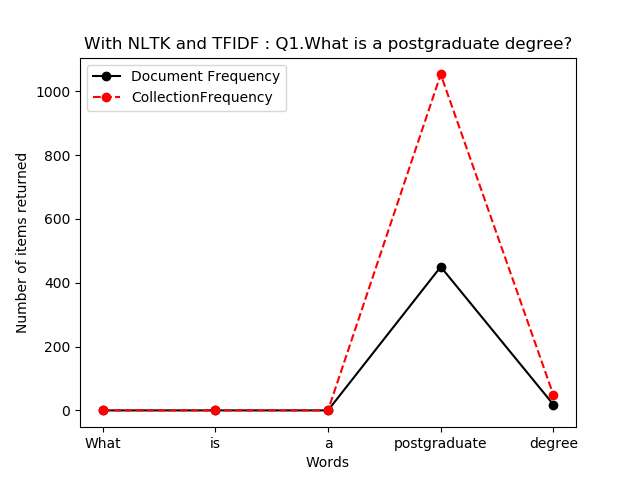
\includegraphics[width=0.4 \textwidth, height=0.16 \textheight] {Q1_everything.PNG}\\
\end{figure}

\begin{figure}[H]
	\centering
	\caption{Without NLTK}\label{fig:dist}
	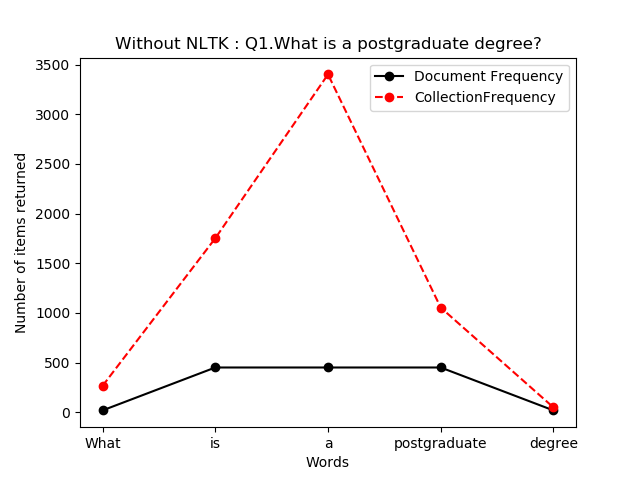
\includegraphics[width=0.4 \textwidth, height=0.16 \textheight] {Q1_NoNLTK.PNG}\\
\end{figure}

The difference in information being returned, between figure 1 and 2, was due to NLTK being removed. This eliminated the system's ability to identify 'stopwords'. These were, therefore, included in the returned data and impacted the weighting relevance of the URL's being returned (see table 1 for the differences).

\begin{figure}[H]
	\centering
	\caption{Without NLTK and TF*IDF}\label{fig:dist}
	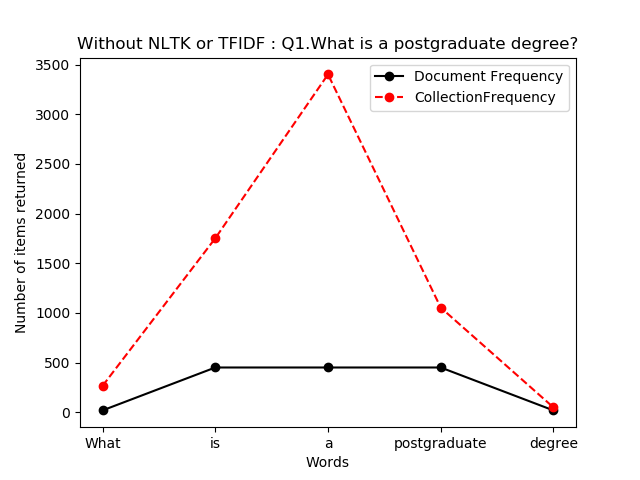
\includegraphics[width=0.4 \textwidth, height=.16 \textheight] {Q1_nothing.PNG}\\
\end{figure}

When TF*IDF was also removed the author found no change between figure 2 and figure 3. This, therefore, took the author one step further to investigate the top 3 URL's being returned for both processes. Even though there was no difference between the number of term and document frequency figures being returned there was a definite difference in relevant URL's being returned (see tables 2 and 3): 

\begin{table} [h]
	\centering 
	\caption{Without NLTK}\label{textresult}
	\begin{tabular}{|l|} \hline
		student-support-service/travel-and-expeditions \\
		postgraduate-research/pgr-regulations-and-forms  \\
		graduationoffice/honorary-graduate-nominations \\
		\hline
	\end{tabular}
\end{table}

\begin{table} [h]
	\centering 
	\caption{Without NLTK and TF*IDF}\label{textresult}
	\begin{tabular}{|l|} \hline
		portal.uea.ac.uk/  \\
		student-support-service/disability  \\
		estates/security \\
		\hline
	\end{tabular}
\end{table}

These differences were due to the TF*IDF ranking the words into priority order and, when removed, the system had no way to process the ranking, so just output the URL's based on the number of times each word was found.

\section{Testing Issues Encountered}
There were a couple of issues encountered during the testing phase: 

As this was a very big website with a lot of information to 'scrape' the crawling process timed out several times before obtaining all the information needed. 

This site, also, produced a massive amount of data within the .txt document files. This meant that using these documents for testing was a very slow process as it could take up to 5 minutes to return the search question and output the relevant URL's. The author decided to complete the testing on a smaller sample of 500 URL's. 

\section{Comparison and Conclusions } \label{comparison}
Once the test questions were analysed the search engine was compared to the search process on the portal site, as well as a list of 'best case' URL's provided by Dan Smith, for 10 questions. Some of the URL's appeared for each question, but the author's system did not always rank them correctly.

This highlighted the importance of each process. REGEX for cleaning the text, TF*IDF for ranking orders, Cosine Similarity for checking similarities across documents and NLTK for removing non-relevant text and changing words into their base format, so they could be read and rated correctly. 

This first attempt at a search engine produced a satisfactory return rate, however, the longer and more complex the question, the less likely to receive the correct URL ranking order. To improve the system would require more time and knowledge, along with better cleaning by REGEX. Even with the changes implemented, some of the text was still lost and this impacted the efficiency of the whole system. 

%

\bibliographystyle{apalike}
\bibliography{IR}  


\end{document}
